\label{chapter:metodo}
\par
Este Capítulo descreve o método proposto neste trabalho, baseado transformações de código para análise de circuitos lógicos descritos em VHDL utilizando 
\textit{Bounded Model Checking}, neste caso o \textit{model checker} ESBMC.

%======================
%Visão geral do método
%======================
\section{Visão geral do método}

\par
O método proposto consiste inicialmente em receber como entrada um circuito lógico descrito em VHDL, onde uma dada propriedade representada em uma assertiva será analisada, as assertivas serão inseridas de automaticamente pelo método ou pelo próprio usuário do método. O código VHDL analisado posteriomente é traduzido para linguagem C e recebe uma instrumentação de código (com funções especificas suportadas pelo método) para a posterior validação do mesmo. O Código em C automaticamente gerado, já instrumentado, será processado e analisado pelo ESBMC de acordo com as assertivas inseridas e ao final é apresentado o resultado. Caso alguma das assertivas seja violada, um contra-exemplo é apresentado ao usuário. Uma visão geral do método proposto é apresentado na \autoref{fig:Fluxo_ferramenta} e nas sessões a seguir serão apresentados cada etapa do método proposto neste trabalho.

\begin{figure}[H]
	\begin{center}
    \caption{\label{fig:Fluxo_ferramenta}Ciclo da ferramenta}
	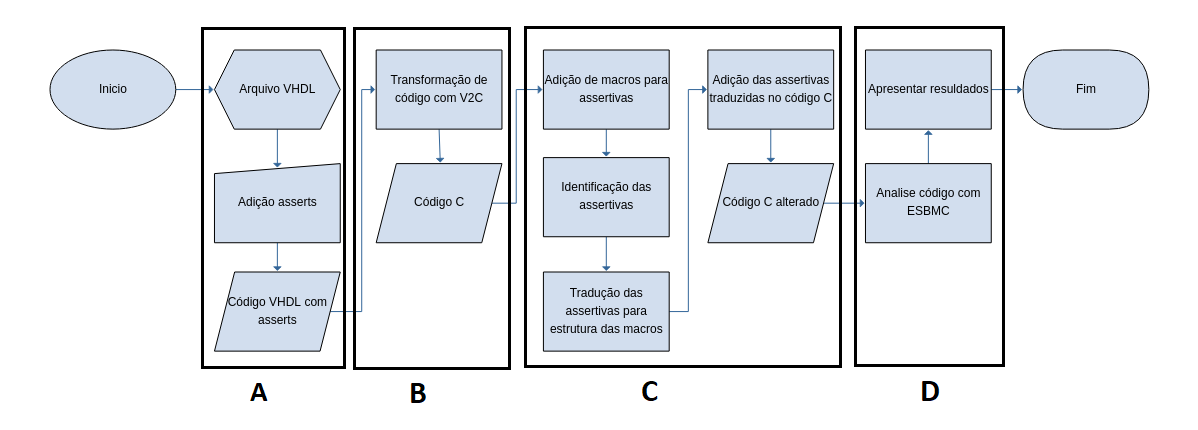
\includegraphics[scale=0.55]{Figuras/Fluxo_ferramenta.png}
	\end{center}
    \legend{Fonte: Própria}
\end{figure}

\par
Com o intuito de auxiliar nas explicações apresentadas nas próximas seções, o código na \autoref{fig:code_exemplo} será utilizado nas explanações, bem como será apresentado todas as alterações do mesmo, conforme cada etapa do método.  

\begin{figure}[H]
\caption{\label{fig:code_exemplo} Exemplo de código VHDL de ULA com portas \texttt{AND}, \texttt{OR} e \texttt{XOR}.}
	\begin{center}
    \begin{minipage}{0.7\textwidth}
    \begin{lstlisting}       
library ieee;
use ieee.std_logic_1164.all;

ENTITY Ula_tcc IS
PORT(A,B,Binvertido,Op1,Op2:IN BIT;
	  Resultado:OUT BIT);
END Ula_tcc;

ARCHITECTURE Ula_tcc_behavl OF Ula_tcc IS
SIGNAL and_port, or_port: bit;
SIGNAL xor_port, mux2x1 :bit;
BEGIN
	PROCESS(A,B,Binvertido,Op1)
	BEGIN
		--PORTA AND
		IF(A = '1' and mux2x1 = '0') THEN
		    and_port <= '1';
		ELSE
		    and_port <= '0';
		END IF;
		--PORTA OR
		IF(A = '0' and mux2x1 = '0') THEN
		    and_port <= '0';
		ELSE
		    and_port <= '1';
		END IF;
		--PORTA XOR
		IF(A = '0' and mux2x1 = '0') THEN
		    xor_port <= '0';
		ELSIF(A = '1' and mux2x1 = '1') THEN
		    xor_port <= '0';
		ELSE
		    xor_port <= '1';
		END IF;
		--INVERSOR
		IF(Binvertido = '0') THEN
			mux2x1 <= B;
		ELSE
			mux2x1 <= NOT B;
		END IF;
		--MUX4X1
		IF(Op1 = '0' and Op2 = '0') THEN
			Resultado <= and_port;
		ELSIF(Op1 = '0' and Op2 = '1') THEN
			Resultado <= or_port;
		ELSIF(Op1 = '1' and Op2 = '0') THEN
			Resultado <= xor_port;
		END IF;
	END PROCESS;
END Ula_tcc_behavl;
    \end{lstlisting}
    \end{minipage}
	\end{center}
    \legend{Fonte: Própria.}
\end{figure}

\textcolor{red}{O código apresenta um erro na \textbf{linha 18} e este é o ponto principal para análise do código e estudo do método. Na tabela verdade da porta AND, para que o valor resultado seja 1 é necessário que ambas as entradas seja 1, no código é apresentado entradas 1 e 0 para o resultado 1, assim tendo um erro de código.}

%========================
%Preprocessamento do VHDL e inserção de assertivas
%========================
\section{Preprocessamento do VHDL e inserção de assertivas}
\label{cap:vhdl_assertivas}

\par
A fase inicial do método consiste no pré-processamento do código VHDL com as anotações de código pelo usuário ou pelo método proposto de forma automática, incluindo as assertivas, conforme a \autoref{fig:Fluxo_ferramenta}, na \textbf{etapa A}. O método não realiza qualquer tipo de verificação sobre o código VHDL, apenas utiliza o mesmo como entrada juntamente com as assertivas inseridas. Toda verificação é realizada sobre o código em linguagem C, que será traduzido a partir do código VHDL analisado, nas próximas etapas do método proposto. Vale ressaltar que mesmo a linguagem VHDL tendo um modelo de assertivas padrão, para o método tornou-se necessário a criação de um modelo (baseado em comentários) para que as funções do model checker adotado fossem suportadas, como a geração de valores não deterministicos.

\par
\label{sec:assertiva_descricao} As assertivas manuais são adicionadas entre as tags \texttt{@c2vhdl:ASSERT} e \texttt{@c2vhdl:END} e todo trecho de código entre estas tags deve estar comentado, desta forma não apresentará erro na tradução do código em linguagem C, bem como na sintetização do código VHDL. Nas assertivas são incluidas as funções necessárias para a análise utilizando a ferramenta ESBMC. A assertiva apresenta três informações principais, sendo elas: condição, mensagem e gravidade.

\begin{figure}[H]
\caption{\label{fig:assertiva} Exemplo de assertiva para verificação de porta \texttt{XOR}.}
	\begin{center}
    \begin{minipage}{0.99\textwidth}
    \begin{lstlisting}       
--@c2vhdl:ASSERT
--assert (Resultado = '1')
--report "O resutado foi diferente de 0"
--severity ERROR;
--@c2vhdl:END
    \end{lstlisting}
    \end{minipage}
	\end{center}
    \legend{Fonte: Própria.}
\end{figure}

\par
A condição\textcolor{red}{, \textbf{linha $2$} da \autoref{fig:assertiva},} representa a assertiva propriamente dita e que será analisado pela aplicação. A condição será precedida de \texttt{$--$assert} e seguido ou não da palavra \texttt{not}, com isso a assertiva pode assumir valor negativo, conforme necessidade do usuário. Na \autoref{fig:assertiva} a assertiva busca verificar se a variável \texttt{Resultado} terá valor igual a $1$, com isso ao comparar o valor buscado pela assertiva e o gerado não final do código, ambos serão iguais, gerando a falha na verificação.

\par
A mensagem\textcolor{red}{, \textbf{linha $3$} da \autoref{fig:assertiva},} é definida pelo usuário e será exibida caso a assertiva apresente falha, assim a mensagem pode ser utilizada como um meio de depuração das propriedades validadas. A severidade\textcolor{red}{, \textbf{linha $2$} da \autoref{fig:assertiva},} pode ser definida como \texttt{error}, que representa um erro fatal e parada da verificação. A severidade do tipo \texttt{warning} que representa um erro não fatal, contabiliza as falhas das assertivas, porém não causa a parada da verificação. As mensagens futuramente pode ser integradas um framework para teste de unidade, contudo está é uma etapa ainda em planejamento neste trabalho.

\par
Juntamente com as assertivas outra função que pode ser utilizada é a função \texttt{\_\_ESBMC\allowbreak{}\_assume()} suportada pelo model checker ESBMC. Esta função utilizada em conjuto com a ferramenta ESBMC permite que durante a verificação uma variavél possa ter uma valor setado durante o tempo de execução da verificação. A importância desta função é fazer verificações onde se conhece os valores de entrada juntamente com o valor resultante, por exemplo, na verificação de portas lógicas.

\begin{figure}[H]
\caption{\label{fig:assertiva_assume} Exemplo de utilização da função \texttt{\_\_ESBMC\_assume()}.}
	\begin{center}
    \begin{minipage}{0.99\textwidth}
    \begin{lstlisting}       
    --__ESBMC_assume(A = '1')
    --__ESBMC_assume(mux2x1 = '0');
    \end{lstlisting}
    \end{minipage}
	\end{center}
    \legend{Fonte: Própria.}
\end{figure}

\par
A assertivas que serão verificadas são automáticas traduzidas a partir das entradas do código VHDL. Seja no modelo manual (assertivas escritas pelo usuário) ou automático (inferidas pelo método proposto por meio de análise estática), as entradas são mapeadas para serem utilizados na etapa de instrumentação. Desta forma, tais entradas podem ser utilizadas para gerar essas assertivas e então serem adicionadas diretamente ao código em linguagem C durante a fase de instrumentação.

\par
A \autoref{fig:code_exemplo_assertiva} apresenta o código juntamente com as assertivas conforme o padrão salientado na \autoref{sec:assertiva_descricao}. Neste exemplo foi implementado utilizado a inserção manual das assertivas e também da função \texttt{\_\_ESBMC\_assume()}, entretanto o objetivo é automatizar estas funções durante a execução da ferramenta.

\begin{figure}[H]
\caption{\label{fig:code_exemplo_assertiva} Código da \autoref{fig:code_exemplo} com a assertiva da \autoref{fig:assertiva}.}
	\begin{center}
    \begin{minipage}{0.99\textwidth}
    \begin{lstlisting}       
library ieee;
use ieee.std_logic_1164.all;
...
ARCHITECTURE Ula_tcc_behavl OF Ula_tcc IS
SIGNAL and_port, or_port: bit;
SIGNAL xor_port, mux2x1:bit;
BEGIN
	PROCESS(A,B,Binvertido,Op1) IS
	BEGIN
		--PORTA AND
		IF(A = '1' and mux2x1 = '0') THEN
    --__ESBMC_assume(A = '1')
    --__ESBMC_assume(mux2x1 = '0');
		    and_port <= '1';
		ELSE
		    and_port <= '0';
		END IF;
		...
		--MUX4X1
		IF(Op1 = '0' and Op2 = '0') THEN
			Resultado <= and_port;
		ELSIF(Op1 = '0' and Op2 = '1') THEN
			Resultado <= or_port;
		ELSIF(Op1 = '1' and Op2 = '0') THEN
			Resultado <= xor_port;
        --@c2vhdl:ASSERT
        --assert (Resultado = '1');
        --report "O resutado foi diferente de 0";
        --severity ERROR;
        --@c2vhdl:END
		END IF;
	END PROCESS;
END Ula_tcc_behavl;
    \end{lstlisting}
    \end{minipage}
	\end{center}
    \legend{Fonte: Própria.}
\end{figure}
%===================================
%Tradução para código em linguagem C
%===================================
\section{\label{cap:traducao}Tradução de código VHDL para a linguagem C}

\par
Nesta etapa a tradução do código VHDL para linguagem C é executada, conforme apresentado na \autoref{fig:Fluxo_ferramenta}, \textbf{etapa B}. A partir deste ponto, a ferramenta é executada de maneira propriamente dita, tendo todo o processo automatizado até a apresentação do resultado. Para esta etapa do método foi selecionado a ferramenta V2C\cite{albertoV2C} que realiza a tradução de VHDL para Linguagem C.

\par
A ferramenta V2C apresenta diversas vantagens em relação a equivalência de tradução de linguagens, contudo V2C apresenta certas limitações na tradução do código VHDL, em outras palavras, a mesma não reconhece algumas estruturas específicas do VHDL. A ferramenta aceita apenas entradas e saídas do tipo: \texttt{bit}, \texttt{std\_ulogic}, \texttt{qsim\_state}, \texttt{std\_ulogic\_vector} e \texttt{interger}. Na parte de arquitetura, a ferramenta aceita uma gama maior de estruturas, trabalhando com expressões do tipo: \texttt{signal}, \texttt{variable}, \texttt{integers}, \texttt{strings} e caracteres. Em expressões condicionais os operandos são \texttt{AND}, \texttt{OR}, \texttt{NOT} $<=$, $=>$,$=$,$<$,$>$ e $<>$. Aceita também a estrutura de \texttt{process}, além da estrutura \texttt{block}. A estrutura \texttt{process} é limitada apenas a: \texttt{if-else}, \texttt{case} e \texttt{loops}. Como trabalho futuro, neste trabalho tem-se buscado novas abordagens para ampliar o suporte a estruturas não suportadas pelo V2C.

\par
Na tradução é necessário substituir os operadores originais por seus equivalentes em linguagem C. A exceção são os operadores específicos que gerenciam os valores de \texttt{bit}, tais como concatenação ou manipulação de partes vetores, para os quais são necessários construir procedimentos específicos em C.

Conforme mostrado na \autoref{fig:code_traduzido}, na tradução são gerados vários vetores para suporte a tradução dos sinais representados no VHDL, sendo eles \texttt{chg[]}, \texttt{old[]} e \texttt{new[]}. \textcolor{red}{O vetor \texttt{old[]} contém o valor dos sinais do ciclo anterior e operação e a partir deste vetor, o valor a ser usado nos cálculos posteriores é obtido. O vetor \texttt{new[]} representa os novos valores que foram calculados durante a execução do ciclo e este novos são calculados pelos antigos existentes no vetor \texttt{old[]}. E o vetor \texttt{chg[]} contém um or exclusivo entre o valor novo e antigo e em caso de alteração entre os valores é copiado o valor de \texttt{new[]} para \texttt{old[]}.}

\par
No código C gerado, os vetores \texttt{in\_data[]} e \texttt{out\_data[]} contêm os sinais de entrada e saída, respectivamente. \textcolor{red}{No caso de circuitos sequenciais, o valor do status é inserido no primeiro (índice 0). A ferramenta lerá os valores \texttt{in\_data[]} e escreverá os resultados do processamento em \texttt{out\_data[]}. Ao final da operação os valores de estado finais salvos no vetor \texttt{new[]} são passado para \texttt{out\_data[]}.}

\par
Conforme especificado e seguindo os parâmetros da ferramenta, a mesma realiza a tradução, mantendo inalterado qualquer fragmento de código que esteja comentado, neste caso, as assertivas presentes no código VHDL permanecem inalteradas, sendo utilizadas na próxima etapa do método proposto.

\begin{figure}[H]
\caption{\label{fig:code_traduzido} Código da \autoref{fig:code_exemplo} traduzido pela ferramenta V2C.}
	\begin{center}
    \begin{minipage}{0.99\textwidth}
    \begin{lstlisting}      
void ula_tcc(int in_data[], int out_data[]){
...
enum segnale {A, B, Binvertido, Op1, Op2, Resultado, and_port, or_port, xor_port, mux2x1, _MAX_};
int old[_MAX_];
int new[_MAX_];
int chg[_MAX_];
...
do {
   _cont_=0;
   /* Start of Translation */
   if (chg[A] || chg[B] || chg[Binvertido] || chg[Op1]) {
            /*PORTA AND */
      if ((old[A]==1 && old[mux2x1]==0)) {
	   \\__ESBMC_assume(old[A] = 1);
           \\__ESBMC_assume(old[mux2x1] = 0);
         new[and_port]=1;
         }
      else {
         new[and_port]=0;
         }
      ...
      /*MUX4X1 */
      if ((old[Op1]==0 && old[Op2]==0)) {
         if (chg[and_port]) {
            new[Resultado]=old[and_port];
	    \\@c2vhdl:ASSERT
            \\assert (Resultado = '1');
            \\report "O resutado foi diferente de 0";
            \\severity ERROR;
            \\@c2vhdl:END
            }
         }
      else if ((old[Op1]==0 && old[Op2]==1)) {
         if (chg[or_port]) {
            new[Resultado]=old[or_port];
            }
         }
      else if ((old[Op1]==1 && old[Op2]==0)) {
         if (chg[xor_port]) {
            new[Resultado]=old[xor_port];
            }
         }
      }
   /* End of Translation */
...
}
    \end{lstlisting}
    \end{minipage}
	\end{center}
    \legend{Fonte: Própria.}
\end{figure}

%========================
%Instrumentação de código
%========================
\section{Instrumentação de código}

\par
As assertivas após a tradução permanecem comentadas, sendo necessário preparar-las, ou seja traduzi-las, para verificação posterior do código na linguagem em C. Com isso é necessário uma instrumentação do código para prover suporte as assertivas traduzidas para análise, conforme apresentado na \autoref{fig:Fluxo_ferramenta}, \textbf{etapa C}.

\par
Todas as etapas da instrumentação são realizados sobre o código C já traduzido. O passo inicial da instrumentação é a adição da macros no início do código C com as definição das assertivas a serem utilizadas. Na \autoref{fig:macro} são apresentados os macros utilizadas no código C. A Linha $1$ da figura corresponde a mensagem de erro a ser apresentada e a Linha $2$ corresponde ao modelo da assertiva e a chamada da macro definida na Linha $1$ em caso de falha. Estas definições para as assertivas também podem ser utilizadas no código C traduzidos sem o uso do ESBMC.


\begin{figure}[H]
\caption{\label{fig:macro} Macros das assertivas implementadas em linguagem C}
	\begin{center}
    \begin{minipage}{0.99\textwidth}
    \begin{lstlisting}       
#define log_error(M,...)fprintf(stderr,M,__FILE__,__LINE__,##__VA_ARGS__)
#define __MY_assert(A, M,...) if(!(A)) {log_error(M, ##__VA_ARGS__); assert(A); }
    \end{lstlisting}
    \end{minipage}
	\end{center}
    \legend{Fonte: Própria.}
\end{figure}

\par
O passo seguinte é a identificação das assertivas comentadas ao longo do corpo do código traduzido, utilizando o exemplo da \autoref{fig:assert_c}. As assertivas são identificadas através das tags \texttt{@c2vhdl:ASSERT} e \texttt{@c2vhdl:END} e a busca é realizado através destas tags. Ao ser encontrado a tag \texttt{@c2vhdl:ASSERT}, é realizado um \textit{loop} até que seja encontrada a tag \textbf{@c2vhdl:END} e com isso toda a assertiva inserida possa ser passada a função de busca das informações da assertiva contidas entre as tags apresentadas.

\par
Com os dados das assertivas obtidos é realizado a busca da condição, mensagem e severidade através dos comandos \texttt{$--$assert}, \texttt{$--$report} e \texttt{$--$severity} respectivamente. Estas informações são encontradas através do uso e uma Regex no código e que são adicionadas ao código C seguindo o modelo definido na macro. Este processo é repetido até outra assertiva ser encontrada ou caso chegue ao final do código C.

\par
Com a função \texttt{\_\_ESBMC\_assume()} ocorre processo semelhante ao das assertivas. Utilizando novamente uma regex que realiza a busca por esta função no código e é retirado o comentário da mesma, desta forma a mesma passa a esta acessível para o ESBMC, visto que a declaração da mesma já segue o modelo padrão a ser utilizado pelo ESBMC.

\par
Durante a instrumentação de código também é realizado a entrada de sinais não determinísticos para variáveis não inicializadas ou argumentos de funções do código C gerado da tradução, utilizando a função \texttt{\_\_VERIFIER\_nondet\_int()}. Esta função é utilizada em todas as variáveis de entrada e também nos sinais criados ao longo da arquitetura. Desta forma, todas as variáveis necessárias são inicializadas para verificação.

\par
Segundo, \citeonline{rocha2015verificaccao}, a função \texttt{\_\_VERIFIER\_nondet\_int()} tem a função de modelar valores inteiros não determinísticos e é importante no desenvolvimento do método, pois evita erros, onde dado estado do código não pode ser alcançado, devido a variável não inicializada.

\begin{figure}[H]
\caption{\label{fig:assert_c} Código com assertivas traduzida para linguagem C}
	\begin{center}
    \begin{minipage}{0.99\textwidth}
    \begin{lstlisting}       
#include<stdio.h>
#define log_error(M, ...) fprintf(stderr,  M , __FILE__, __LINE__, ##__VA_ARGS__)//Update to print the trace
#define __MY_assert(A, M, ...) if(!(A)) {log_error(M, ##__VA_ARGS__); assert(A); }

...

do {
   _cont_=0;
   /* Start of Translation */
    chg[A] = __VERIFIER_nondet_int(); 
    chg[B] = __VERIFIER_nondet_int(); 
    chg[Binvertido] = __VERIFIER_nondet_int(); 
    chg[Op1] = __VERIFIER_nondet_int();
    chg[and_port] = __VERIFIER_nondet_int();
    chg[Resultado] = __VERIFIER_nondet_int();
    chg[or_port] = __VERIFIER_nondet_int();
    chg[mux2x1] = __VERIFIER_nondet_int();

   /* p0: */
   if (chg[A] || chg[B] || chg[Binvertido] || chg[Op1]) {
            /*PORTA AND */
      if ((old[A]==1 && old[mux2x1]==0)) {
	   __ESBMC_assume(old[A] = 1);
           __ESBMC_assume(old[mux2x1] = 0);
         new[and_port]=1;
         }
      else {
         new[and_port]=0;
         }

      ...

      /*MUX4X1 */
      if ((old[Op1]==0 && old[Op2]==0)) {
         if (chg[and_port]) {
            new[Resultado]=old[and_port];
	    __MY_assert(new[Resultado] == 1,"O resultado é diferente de 0");
         }
      else if ((old[Op1]==0 && old[Op2]==1)) {
         if (chg[or_port]) {
            new[Resultado]=old[or_port];
            }
         }
      else if ((old[Op1]==1 && old[Op2]==0)) {
         if (chg[xor_port]) {
            new[Resultado]=old[xor_port];
            }
         }
      }

   /* End of Translation */
...
    \end{lstlisting}
    \end{minipage}
	\end{center}
    \legend{Fonte: Própria.}
\end{figure}

\par
Em outras palavras, na instrumentação de código é realizado a tradução das assertivas do modelo utilizado no código VHDL para para o modelo utilizado em linguagem C, além como de outras funções que possam ser utilizados pelo VHDL. Ao final da instrumentação o código C fica disponível para que possa ser dado como entrada para outras ferramentas de verificação de código e não apenas o ESBMC.

%=============================================
%Verificação de assertvas usando model checker
%=============================================
\section{Verificação de assertivas usando \textit{Model Checker}}

\par
O \textit{model checker} adotado no desenvolvimento de método é o ESBMC~\cite{cordeiro2012smt} na versão $3.0.0$ e conforme explicado na \autoref{cap:bounded}, esta ferramenta recebe como entrada um código C ou C$++$ \textcolor{red}{e também utiliza solucionadores SMT para análise} e devido a isso foi escolhida neste projeto. Nesta seção será apresentado a \textbf{etapa D} do método proposto na \autoref{fig:Fluxo_ferramenta}.

\par
Para a verificação, a primeira etapa é a identificação das assertivas no código C analisado, para isso é utilizado uma opção do ESBMC (\texttt{$--$show-claims}), mais especificamente as assertivas instrumentadas no código C analisado. Cada assertiva é identificada através de uma numeração de acordo com a ordem de busca do código analisado. Cada assertiva encontrada é armazenada para que seja realizada uma análise individual de cada \textit{claim}, ou seja,  assertiva.


\begin{figure}[H]
\caption{\label{fig:codigo_claims} Código apresentando a função de busca das clains com assertivas.}
	\begin{center}
    \begin{minipage}{0.99\textwidth}
    \begin{lstlisting}       
VAR
  contador: 	inteiro
  claim: 	lista
  claim_string: string 

FUNCAO call_esbmc: arquivo
  contador<-0
  INICIO
  saida<-funcao de geracao das claims pelo ESBMC
  ENQUANTO contador < saida FACA
    contador+=2
    regex para procurar claim e numeracao da claim
    SE encontrar claim ENTAO
      regex para procurar a palavra "assertion"
      SE encontrar a palavra "assertion" ENTAO
        contador+=1
	Adiciona a numeracao da claim na lista
      FIM-SE
    FIM-SE
  FIM-ENQUANTO
FIM-FUNCAO
    \end{lstlisting}
    \end{minipage}
	\end{center}
    \legend{Fonte: Própria.}
\end{figure}

\par
Na Linha $9$ da \autoref{fig:codigo_claims} é apresentado a chamada da ferramenta ESBMC que ocorre e através da opção \texttt{$--$show-claims} lista todas as claims presentes no texto, como apresentado na \autoref{fig:claims_assertivas}. Como o ESBMC infere de forma automática assertivas a serem verificadas no código. Visando isolar somente as assertivas instrumentadas pelo método proposto, juntamente com a opção \textit{--show-claims} é utilizado as opções:
\begin{itemize}
    \item \texttt{$--$no-pointer-check:} para não realizar a checagem de ponteiros no código;
    \item \texttt{$--$no-div-by-zero-check:} para não realizar a checagem de divisões por zero no código; e
    \item \texttt{$--$no-bounds-check:} para não realizar a checagem de array bounds no código.
\end{itemize}

\begin{figure}[H]
	\begin{center}
    \caption{\label{fig:claims_assertivas}Imagem de claims contendo assertivas.}
	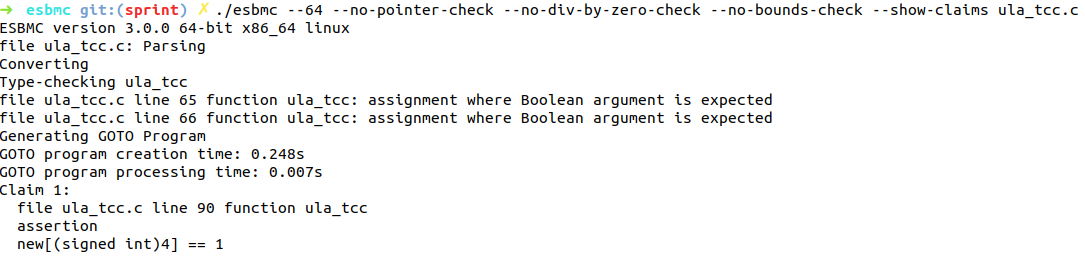
\includegraphics[scale=0.55 ]{Figuras/lista_claim.png}
	\end{center}
    \legend{Fonte:Própria}
\end{figure}

\par
Após a listagem das claims com assertivas ser gerada, outra função, indicada na \autoref{fig:analise_claims}, é chamada para verificação de cada claim individualmente. Para cada claim, ocorre a chamada do ESBMC, utilizando as opções \texttt{$--$no-pointer-check}, \texttt{$--$no-div-by-zero-check} e \texttt{$--$no-bounds-check}, juntamente com a opção \texttt{$--$unwind} em que realiza o número de desdobramentos dos laços no código analisado. 

\par
Contudo, dependendo da complexidade da assertiva, faz-se necessário aumentar o número de desdobramentos que, por padrão são dez, conforme análise experimentais. A função é chamada na Linha $11$ da \autoref{fig:analise_claims} e após a análise da claim é realizado a busca do resultado e exibição caso seja uma propriedade violada.

\par
Desta forma o ESBMC realiza apenas a checagem necessária dentro da assertiva, evitando que outros parâmetros sejam verificados, sem a devida necessidade do mesmo. Ao final de todos os desdobramentos é apresentado o resultado, apresentado na \autoref{fig:resultado}, sendo positiva (sem erros) ou negativa (com violação de propriedades), dependendo da assertiva e do código analisado. Este processo se repete até a lista de assertivas ser finalizada.

\begin{figure}[H]
\caption{\label{fig:analise_claims}Pseudocódigo da função de análise das claims.}
	\begin{center}
    \begin{minipage}{0.7\textwidth}
    \begin{lstlisting}       
VAR
contador1: inteiro
contador2: inteiro
resultado: lista

FUNCAO esbmc_claims: lista, arquivo
  contador1<-0
  contador2<-0
  busca pelo nome da funcao no arquivo
  ENQUANTO contador < lista FACA
    saida<-Executa comando de analise da claim numerada na lista
    ENQUANTO contador2 < saida
      Regex busca se a propriedade foi violada
      SE propriedade foi violada ENTAO
         Pula para linha da violação
	       Adiciona o erro ao resultado       
      FIM-SE  
    FIM-ENQUANTO
  FIM-ENQUANTO
FIM-FUNCAO
    \end{lstlisting}
    \end{minipage}
	\end{center}
    \legend{Fonte: Própria.}
\end{figure}

\begin{figure}[H]
	\begin{center}
    \caption{\label{fig:resultado}Imagem de apresentação do resultado da ferramenta.}
	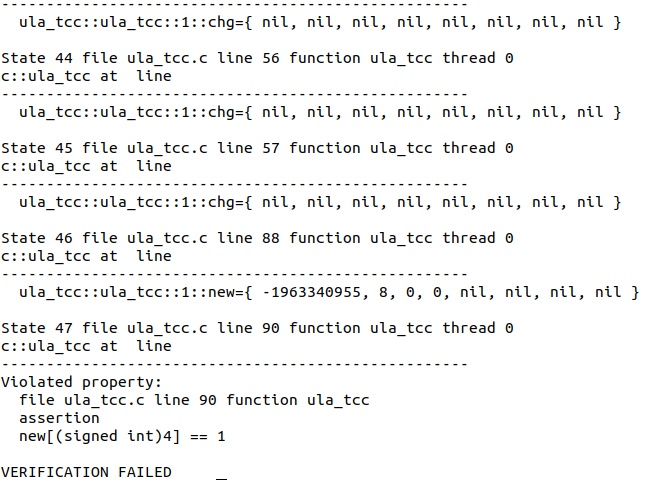
\includegraphics[scale=0.6]{Figuras/erro_assert.png}
	\end{center}
    \legend{Fonte:Própria}
\end{figure}
